\documentclass[12pt]{article}

\usepackage{amssymb,amsmath,amsfonts,eurosym,geometry,ulem,graphicx,caption,color,setspace,sectsty,comment,footmisc,caption,natbib,pdflscape,subfigure,array,hyperref}
\usepackage{indentfirst}

\normalem

\onehalfspacing
\newtheorem{theorem}{Theorem}
\newtheorem{corollary}[theorem]{Corollary}
\newtheorem{proposition}{Proposition}
\newenvironment{proof}[1][Proof]{\noindent\textbf{#1.} }{\ \rule{0.5em}{0.5em}}

\newtheorem{hyp}{Hypothesis}
\newtheorem{subhyp}{Hypothesis}[hyp]
\renewcommand{\thesubhyp}{\thehyp\alph{subhyp}}

\newcommand{\red}[1]{{\color{red} #1}}
\newcommand{\blue}[1]{{\color{blue} #1}}

\newcolumntype{L}[1]{>{\raggedright\let\newline\\arraybackslash\hspace{0pt}}m{#1}}
\newcolumntype{C}[1]{>{\centering\let\newline\\arraybackslash\hspace{0pt}}m{#1}}
\newcolumntype{R}[1]{>{\raggedleft\let\newline\\arraybackslash\hspace{0pt}}m{#1}}

\geometry{left=1.0in,right=1.0in,top=1.0in,bottom=1.0in}

\begin{document}

\begin{titlepage}
\title{Predictions on TARGET2 Balance}
\author{Sherry Peng Tian\thanks{Tian: Boston College, tianpe@bc.edu, Eagle ID: 17651338}}
% \and Surname2\thanks{affiliation2, address2, email2. Acknowledgements}}
\date{\today}
\maketitle
\begin{abstract}
\noindent Placeholder\\
\vspace{0in}\\
\noindent\textbf{Keywords:} key1, key2, key3\\
\bigskip
\end{abstract}
\setcounter{page}{0}
\thispagestyle{empty}
\end{titlepage}

\pagebreak \newpage

\doublespacing

%\clearpage
%\section*{Figures} \label{sec:fig}
%\addcontentsline{toc}{section}{Figures}

%\begin{figure}[hp]
%  \centering
%  \includegraphics[width=.6\textwidth]{../fig/placeholder.pdf}
%  \caption{Placeholder}
%  \label{fig:placeholder}
%\end{figure}
%\clearpage


\section{Background} \label{sec:background}

European Union, as the largest monetary organization and the second largest economy in nominal terms (only after the United States) according to GDP, PPP, and nominal GDP, those normally accepted economic measures, was established in November, 1993. EU countries gather together to make determination on economic policies, environmental issues, political pointviews, and even educational and employment development. Therefore, the study of the EU economy assists in the long run of understanding and predicting the global trend of economic development. Starting from the year of 1999 with some EU member states, now 19 out of 28 EU states/countries accept and use euro as official and main currency in a currency union (called Eurozone); however the remaining 9 states still accept the usage of euro in some ways, making euro the most widely used currency in the EU. 

TARGET2 stands for Trans-European Automated Real-time Gross settlement Express Transfer system and works as a settlement system for the Eurozone. It is based on an integrated central technical infrastructure, called the Single Shared Platform (SSP), which is operated by three central banks of France, Germany, and Italy. Beginning in November 2007, TARGET2 starts to replace TARGET and is made accessible to members outside of the Eurozone countries. Since TARGET2 works as an interbank real-time gross settlement payment system for the clearing of cross-border transfers in the Eurozone, the objectives includes supporting EU monetary policy, stablizing Eurozone money market, minimizing systemic risk and increasing the efficiency of cross-border transfers. Understanding and accurately predicting of TARGET2 balance can establish a good foundation about the global economics. 

Since the Eurozone monetary system consists of the European Central Bank (ECB) and the national central banks of all 19 EU member states, a well-balanced TARGET2 system should be the national commercial banks supporting investment and consumption while maintaining a clear transaction with the national central bank, and then the central banks of different countries linking to ECB via TARGET system, left with parties of creditor nations and borrower nations. When a Eurozone country has a balanced national payment, its TARGET2 balance equals to zero, but when a country encounters unwilingness of equity financing or the expectation of macroeconomics is inclined to drop, the country lacks the capability to pay debts back and becomes the debitor nation, resulting in the creditor nation with a positive TARGET2 balance. During the financial crisis, the After the 2008 financial crisis, the Eurozone monetary market recovers from the higher pressure of subprime financial debts around 2012. 


\section{Literature Review} \label{sec:literature}
\subsection{Interpreting TARGET2 balances}


\subsection{Measuring Economic Policy Uncertainty}
This journal introduces a new index of economic policy uncertainty (EPU) covering major financial events after late 1930s. The approach to establishing indices is based on human-reading newspaper coverage frequency and then captures the policy principals, methods, and outcomes. Meanwhile, the indices include categories such as, the Fed, central banks, interest rate, inflation, and etc, based on differentiation of vocabulary. As for human-readings, the paper evaluates the process at the end with an audit study: the researchers spent six months developing an audit process designed for US EPU indices and another 18 months running a large-scale human audit study to ensure correctness. Additionally, the pilot audit was done with student research assistants, who read and coded randomly selected newspaper articles. 
\subsection{Target2}
\subsection{Policy}
\subsection{Box-Cox Transformation}

\section{Model} \label{sec:model}
\subsection{Data Source and Cleaning}

The policy uncertainty index of various countries is derived directly from \href{https://www.policyuncertainty.com/monetary.html}{\underline{Economic Policy Uncertainty}} website and the target2 balance datasets are from \href{http://www.eurocrisismonitor.com}{\underline{Institute of Empirical Economic Research}} at Osnabrück University, which is a reliable source for tracking TARGET2 balances from Janurary 1987 to June 2019, updated nearly on a monthly basis. 

Since the timelines of two datasets are moduled the same, after year and month, there is no difficulty transferring the combined ones into a time series. Refererring to the raw dataset, there are missing variables only for ECB and Cyprus groups. Table 1 below has shown descriptive details of countries' target2 balance as well as the policy uncertainly index from a macroeconomic perspective. In addition, Figure 1 of uncertainly index has shown that most index lie below 200 with some extreme values extending to 1000. The policy uncertainty is measured using political news and macroeconomic events in 100 percentage. The extreme higher index of United Kingdom and France can be explained by the event of Brexit and the discussion around exiting from the EU. Figure 2 shows the median ranking of Target2 Balance, which corresponds to people's usual understanding. Figure 3 displays the only two negative examples of Austria and Begium, where the balance from 2001 till now has been below zero. 
\begin{table}[!htbp] \centering 
  \caption{Descriptive statistics} 
  \label{} 
  \resizebox{1\textwidth}{!}{
\begin{tabular}{@{\extracolsep{5pt}} ccccc} 
\\[-1.8ex]\hline 
\hline \\[-1.8ex] 
 & mean & sd & min & max \\ 
\hline \\[-1.8ex] 
Austria & -24296.7933783784 & 14674.3237811389 & -46049.49 & 4086.61 \\ 
Belgium & -23289.5541891892 & 19329.5564321393 & -98312.13 & 7687.79 \\ 
Cyprus &  &  &  &  \\ 
ECB &  &  &  &  \\ 
European-News-Index & 154.548700315458 & 66.3208691016548 & 47.6923446655273 & 433.277496337891 \\ 
France & 185.035862158011 & 98.0282374243346 & 30.6203689575195 & 574.633178710938 \\ 
France-News-Index & 185.035862158011 & 98.0282374243346 & 30.6203689575195 & 574.633178710938 \\ 
Germany & 137.807954985816 & 65.0741829256057 & 28.4339847564697 & 454.005432128906 \\ 
Germany-News-Index & 137.807954985816 & 65.0741829256057 & 28.4339847564697 & 454.005432128906 \\ 
Greece & 102.636670389217 & 26.6825469949835 & 47.1814761087496 & 188.704530504278 \\ 
Greece-policy-uncertainty & 123.493935990991 & 60.0910694754914 & 28.63219 & 344.2343 \\ 
Ireland & 121.966938633335 & 55.9441890855816 & 22.9658655600782 & 282.127765252969 \\ 
Italy & 110.990210017642 & 38.5988775008311 & 31.7015342712402 & 241.018203735352 \\ 
Italy-News-Index & 110.990210017642 & 38.5988775008311 & 31.7015342712402 & 241.018203735352 \\ 
Netherlands & 95.8721697437445 & 38.2458191255031 & 27.2133611447053 & 233.73110601772 \\ 
Spain & 109.835684836893 & 32.7956285430677 & 56.2692222595215 & 236.578872680664 \\ 
Spain-News-Index & 112.530257319545 & 57.697184778201 & 23.3175201416016 & 407.419403076172 \\ 
Sweden & 91.4955742387561 & 18.6321694506138 & 53.73406929 & 156.7298215 \\ 
UK & 209.477777781787 & 156.802512055422 & 30.4688014984131 & 1141.79553222656 \\ 
UK-News-Index & 209.477777781787 & 156.802512055422 & 30.4688014984131 & 1141.79553222656 \\ 
\hline \\[-1.8ex] 
\end{tabular}} 
\end{table} 
\begin{figure}
  \centering 
  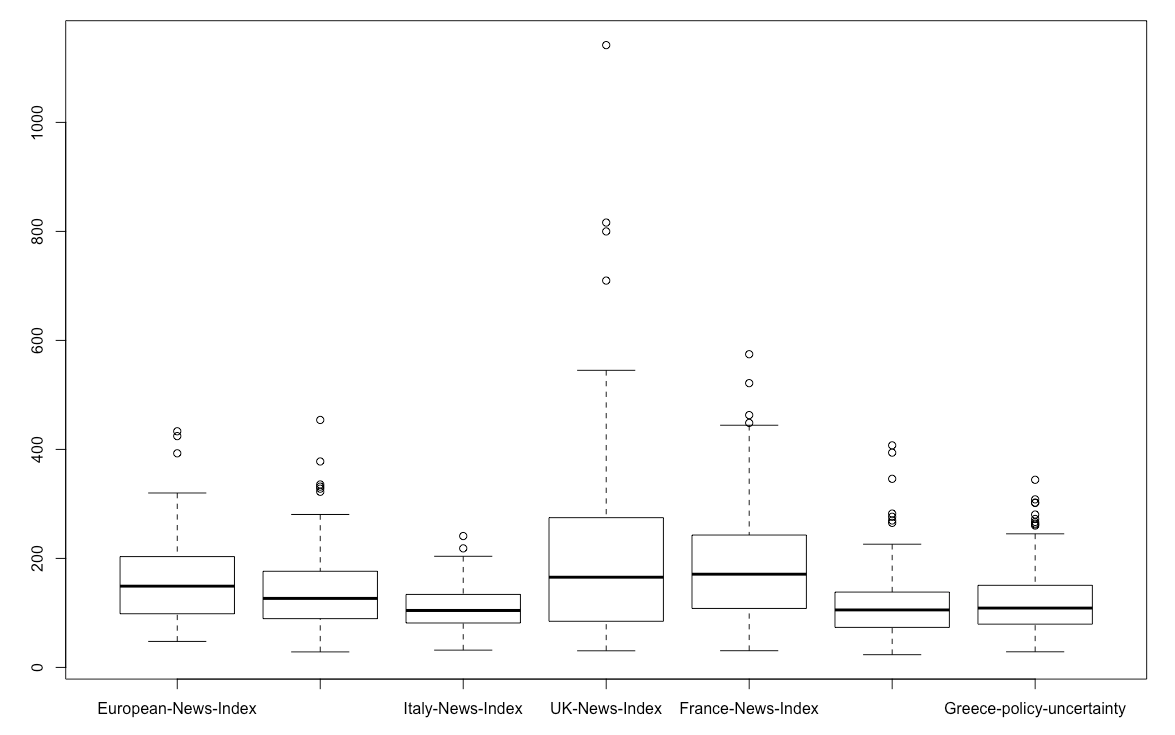
\includegraphics[width=\linewidth]{Uncertainty.png}
  \caption{European, Germany, Italy, UK, France, Spain, Greece News Index}
  \label{fig:policy_uncertainty}
\end{figure}
For the purpose of prediction on Target2 Balance, the time intervals are parsed from the year 2001 because the transition of millennial, even though the financial crisis around 2008 has also seriously influenced the economics and our further prediction. Furthermore, for any need of calculating the accuracy, the test datasest is splitted from Janurary 2015 to June 2019. 
\begin{figure}[!tbp]
  \centering
  \begin{minipage}[b]{0.5\textwidth}
    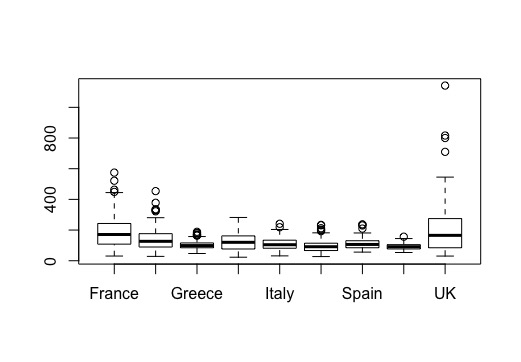
\includegraphics[width=\textwidth]{Bal1.jpeg}
    \caption{Target2 of France, Germany, Greece, Ireland, Italy, Netherlands, Spain, and UK}
  \end{minipage}
  \hfill
  \begin{minipage}[b]{0.4\textwidth}
    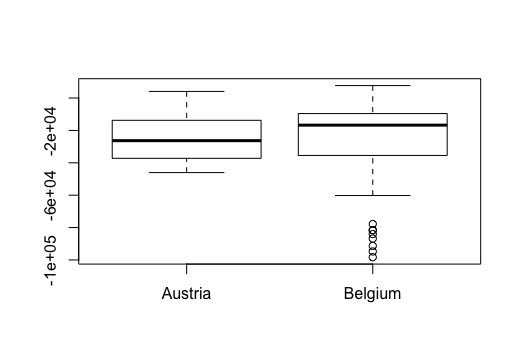
\includegraphics[width=\textwidth]{Bal2.jpeg}
    \caption{Negative Target2 Balance of Austria and Belgium}
  \end{minipage}
\end{figure}
\subsection{Transformation and Decomposition}

Firstly, the additive decomposition of Greece balance from 2001 to June 2019 shows that there might not be a clear trend but there is a clear seasonality occuring every year. Moreover, the multiplicative decomposition shows the same, however, with a smoother trend line. 

\section{Next Things}

%\section{Results} \label{sec:result}

%\section{Conclusion} \label{sec:conclusion}

\singlespacing
\setlength\bibsep{0pt}
\bibliographystyle{my-style}
\bibliography{Placeholder}

\clearpage

\onehalfspacing

\section*{Tables} \label{sec:tab}
\addcontentsline{toc}{section}{Tables}

\section*{Appendix A. Placeholder} \label{sec:appendixa}
\addcontentsline{toc}{section}{Appendix A}

\end{document}